% !TEX encoding = UTF-8
% !TEX TS-program = pdflatex
% !TEX root = ../tesi.tex

%**************************************************************
\chapter{Descrizione dello stage}
\label{cap:descrizione-stage}
%**************************************************************

Il capitolo riporta una descrizione dettagliata dell'attività di stage svolta, analizzando brevemente i possibili rischi, le problematiche da risolvere e le soluzioni proposte. Sono inoltre riportate la pianificazione del lavoro e i requisiti richiesti prima dell'inizio dello stage. 

%**************************************************************
\section{Analisi dei rischi}

Al fine di evitare rallentamenti dei periodi di lavoro è stata effettuata una breve analisi dei
rischi, in modo da poter evitare le situazioni che portano alla creazione di eventi non pianificati,
ove possibile. 

I rischi analizzati sono i seguenti..... TODO

%**************************************************************
\section{Modalità di svolgimento}
L’attività di stage è stata svolta presso la sede dell’azienda per favorire l’interazione dello studente con il tutor e per affacciarlo nella realtà di un team di lavoro aziendale. Lo stagista ha avuto quindi la possibilità di confrontarsi con programmatori più esperti ed essere supportato al meglio in caso di problematiche di sviluppo e gestione del progetto.
Lo studente ha potuto confrontarsi con il tutor per qualsiasi problematica, mentre l’organizzazione settimanale del lavoro è stata gestita tramite dei meeting atti a definire lo stato di avanzamento del progetto e rivedere in tempo reale obiettivi settimanali o miglioramenti del prodotto sulla base dei risultati ottenuti dallo sviluppo.\\ I risultati sono stati valutati settimanalmente (o al termine dell’attività prevista) in base alla quantità e alla qualità dei prodotti forniti dallo studente.
L’orario lavorativo era il seguente: dal lunedì al venerdì dalle 8:40 alle 12:40 e dalle 13:30 alle 17:30.

%**************************************************************
\section{Problematiche da affrontare}
Nella presente sezione sono analizzate, per punti, le problematiche da risolvere attraverso l'attività di stage. (TODO Spiegare più nel dettaglio)

\begin{itemize}
\item Registrazione di una licenza: VISIONEIMPRESA produce un Product Key utilizzando il programma GenPK in base alla tipologia e a un Serial Number casuale, manuale o con le prime due cifre indicanti l’anno. Il Product Key viene aggiunto a un file contenente tutti i Product Key fino ad allora creati, con lo stato “da attivare”, e viene comunicato al cliente. Il cliente all’avvio di Vision è invitato a inserire il Product Key ricevuto, il Software gestionale Vision preleva il MAC Address della scheda di rete su cui sta avvenendo l’installazione e, insieme al Product Key, crea l’Activation Key per verificare successivamente che la licenza sia in uso sulla stessa macchina su cui è stata attivata. Lo stato del Product Key, dopo la registrazione, viene modificato da “da attivare” ad “attivato”. I cambi di stato, la lista dei Product Key e tutte le altre informazioni utilizzate in questo passaggio sono contenute in un file che il Software scarica sul proprio PC tramite protocollo ftp dal server dell’azienda, modifica e rinvia al server. Questa procedura è molto rischiosa, poiché tutte le licenze sono disponibili su un file che potrebbe essere facilmente compromesso.
\item Avvio del Software Gestionale Vision: E’ letta una chiave di registro contenente il Product Key della licenza, viene prelevato il MAC Address e unito al Product Key. Questo codice, che costituisce l’Activation Key, viene controllato con l’Activation Key salvata in locale, e se è uguale allora la macchina utilizzata per accedere è la stessa su cui è stato installato il Software Gestionale Vision, e l’utente può utilizzare il programma normalmente. Poiché il controllo è svolto totalmente in locale è facilmente aggirabile attraverso l’uso di macchine virtuali identiche. Inoltre, un qualsiasi guasto alla scheda di rete costringerebbe il cliente a contattare l’azienda perché, in caso di sostituzione, esso non sarebbe più in grado di utilizzare il Software Gestionale Vision dato che l’Activation Key risultante sarebbe diversa.
\item Caricamento dei moduli della licenza: Il caricamento dei moduli avviene da un file “.HWK”, generato per mezzo del programma GenFileKey, salvato nella cartella del Software Gestionale Vision. Esso contiene un codice cifrato, visibile all’utente, riepilogativo dei moduli attivi della licenza. Questo file può essere facilmente modificato, rischiando di compromettere la licenza. 
\item Licenze bloccate: le licenze bloccate sono contenute in una blacklist all’interno del Software Gestionale Vision, ma nel caso se ne aggiungesse una nuova i clienti dovrebbero aggiornare il programma per avere la black list aggiornata. Se un utente non aggiorna il proprio programma può continuare a utilizzare il programma anche in caso di licenza bloccata. 
\item Procedura di disattivazione: Per disattivare la licenza dal proprio computer e reinstallarla in un altro il cliente è sempre costretto a contattare VISIONEIMPRESA. 
\item Scadenza di una licenza: Le licenze non possiedono una data di scadenza.
\item Rivenditori: I rivenditori per operare, ad esempio per creare una licenza o gestirne i moduli, devono sempre contattare VISIONEIMPRESA.
\item Monitoraggio delle licenze: Monitoraggio minimo fornito da GenPK.

\end{itemize}


%**************************************************************
\section{Soluzioni proposte}

In seguito ai punti salienti esaminati in fase d’analisi, sono proposte (TODO per ora brevemente, da approfondire), per punti, le seguenti soluzioni:
\begin{itemize}

\item	Registrazione di una licenza: In primis si vuole eliminare il sistema dei Product Key salvati in un file, scaricato tramite ftp, costantemente a rischio. La generazione dei Product Key riprenderà il metodo di GenPK, ma i Product Key con le relative caratteristiche saranno salvati su un Database, e la Generazione avverrà tramite Web Service. L’Activation Key viene eliminata e si utilizzerà un nuovo sistema di controllo per l’impronta Hardware, basato su un insieme di componenti e non solo sulla scheda di Rete, in modo da permettere all’utente di cambiare alcune delle componenti del pc (ad esempio in caso di guasti) e non dover ricontattare l’azienda per poter continuare a utilizzare il Software Gestionale Vision. Per la creazione dei Product Key sarà creato un nuovo Software, chiamato License Manager 1.0, che permetterà di creare, gestire e monitorare le licenze in tutti i loro aspetti. Il Software utilizzerà Web Services e Database, eliminando la necessità di affidare file ai clienti con il rischio che siano compromessi. In fase di registrazione il cliente assocerà un indirizzo email alla propria licenza, in modo che possa disattivare e reinstallare il programma senza il bisogno di dover contattare l’azienda.
\item	Avvio del Software Gestionale Vision:  Sono stati pensati due diversi controlli, uno per un accesso senza connessione un per l’accesso con connessione. Il controllo per l’avvio del software in offline utilizzerà informazioni salvate in chiavi di registro per verificare la validità della licenza. E’ stato pensato anche un metodo basato sulle firme digitali per verificare l’integrità delle chiavi di registro. L’utilizzo del programma in offline sarà permesso per 15 giorni, dopo di ché verrà chiesto di connettersi a internet. Il controllo online avviene in due passaggi: uno all’avvio che controlla la validità della licenza in termini di data di scadenza, bloccaggio e componente Hardware, sempre tramite Web Service, e il secondo che si esegue a intervalli regolari di un’ora per verificare che l’utente non stia utilizzando il programma su macchine differenti ma con stesso Hardware (ad esempio clonando una macchina virtuale).
\item	Caricamento dei moduli della licenza: Il codice cifrato verrà salvato in un database, eliminando la necessità di inviare un file ai clienti, con possibilità che esso venga corrotto. La generazione del file che prima avveniva tramite GenFileKey ora sarà possibile eseguirla da License Manager 1.0.
\item	Licenze bloccate: salvando i dati della licenza su un database è facile segnalarne il blocco in uno dei suoi campi. Al momento dei controlli quel campo sarà analizzato, e in caso di blocco presente si deciderà che operazione intraprendere. 
\item	Procedura di disattivazione: associando un indirizzo email alla propria licenza l’utente sarà in grado di disattivare/reinstallare la propria licenza ogni volta che lo vorrà, senza contattare l’azienda e in qualsiasi situazione, anche in caso di rottura del pc o reinstallazione del sistema operativo.
\item	Scadenza di una licenza: sarà implementato un controllo sulla data di scadenza, sia in offline sia in online. Nel controllo all’avvio del programma sarà anche controllato se la licenza è entrata nell’ultimo mese di validità. In quel caso sarà mostrato un reminder con i giorni rimanenti prima della scadenza. 
\item	Rivenditori: License Manager 1.0, grazie al suo sistema di utenti, potrà essere distribuito ai rivenditori con utenti di tipo Guest, lasciando loro un certo grado di libertà che non li costringa a rivolgersi all’azienda per ogni decisione. Ogni azione da loro intrapresa sarà comunicata all’azienda tramite email, e tutti gli stati precedenti alle modifiche saranno registrati in una tabella dedicata del database.
\item	Monitoraggio delle licenze: License Manager 1.0 fornisce un sistema di monitoraggio basato su: visione immediata di tutte le caratteristiche di una licenza, statistiche sulla distribuzione e l’utilizzo delle licenze, log degli accessi al Software Gestionale Vision per notare possibili anomalie.


\end{itemize}

%**************************************************************
\section{Pianificazione del Lavoro}

La seguente sezione mostra la pianificazione del lavoro attuata prima di iniziare l'attività di stage e l'effettivo utilizzo delle ore. Per rendere più chiara la pianificazione del lavoro e lo svolgimento effettivo delle attività sono utilizzati Diagrammi di Gantt.

\subsection{Pianificazione antecedente lo stage}

TODO METTERE IN VERTICALE
\begin{figure}[!h] 
    \centering 
    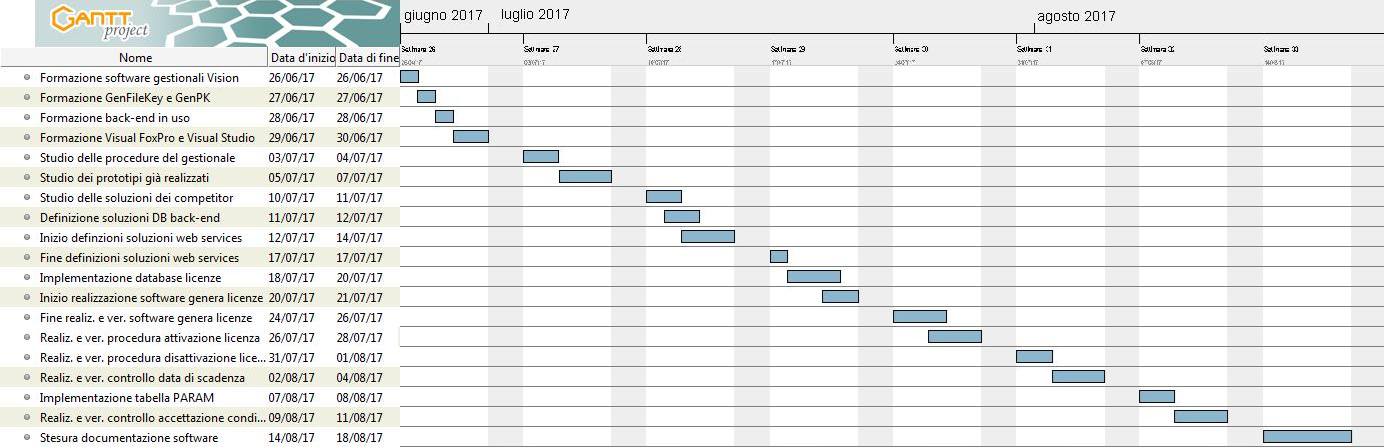
\includegraphics[width=0.9\columnwidth]{ganttPrima} 
    \caption{Diagramma di Gantt - Pianificazione del lavoro}
\end{figure}

\subsection{Resoconto delle attività svolte}

TODO Diagramma post stage

%**************************************************************
\section{Obiettivi e Requisiti}

\subsection{Obiettivi}
Nella fase preliminare dello stage sono stati delineati i seguenti obiettivi, in ordine di importanza. Gli obiettivi sono identificati da un codice così composto: XXYY dove XX rappresenta la tipologia dell'obiettivo (es. OP obiettivo primario) e YY è un numero progressivo.
Le sigle sono queste.. TODO: sigle, espandere e spiegare nel dettaglio gli obiettivi.
\begin{itemize}

\item \textbf{obiettivi primari:}\begin{itemize}
\item OP01: definizione delle strategie risolutive per le problematiche presentate;
\item OP02: implementazione di un sistema di attivazione/disattivazione licenze via web services.
\end{itemize}
\item \textbf{obiettivi secondari:}\begin{itemize}
\item OS1: implementazione della data di scadenza di una licenza e relativi controlli (prototipo da completare).
\end{itemize}
\item \textbf{obiettivi facoltativi:}\begin{itemize}
\item OF01: implementazione licenze per moduli;
\item OF02: raccolta dati sull’attivazione delle licenze e loro utilizzo;
\item OF03: creazione dashboard con statistiche e alert su licenze in uso, disattivate, anomalie.
\end{itemize}
\item \textbf{obiettivi formativi:}\begin{itemize}
\item FO01: acquisizione di competenze utili allo sviluppo di software gestionale;
\item FO02: interazione con un team di lavoro aziendale;
\item FO03: ottenimento di capacità decisionali sulle migliori tecnologie da utilizzare in diversi contesti.
\end{itemize}

\end{itemize}

Durante lo svolgimento dello stage, dopo aver raggiunto tutti gli obiettivi prefissati, è stato posto come obiettivo ultimo la distribuzione del Software License Manager 1.0 anche ai rivenditori dell'azienda.

\subsection{Requisiti}

In relazione agli obiettivi presentati nel paragrafo precedente, sono stati identificati i requisiti riportati in seguito.

\subsubsection{Requisiti OP01}
Per raggiungere una completa (riassunto dell'obiettivo) sono stati identificati i seguenti requisiti:
descrizione dei requisiti da soddisfare per raggiungere l'obiettivo.
\subsubsection{Requisiti OP02} 
Per implementare un efficiente sistema di attivazione sono stati identificati i seguenti requisiti:
\begin{itemize}
\item l'utente finale deve poter inserire all'avvio del Software Gestionale Vision il Product Key, ricevuto in fase d'acquisto, relativo alla licenza per lui creata;
\item il Product Key inserito deve essere controllato tramite un metodo di un Web Service, che provvederà a verificare la disponibilità dello stesso e a impostare le informazioni di attivazione della licenza nella tabella \texttt{Licenze} del database \texttt{DBLicenze};
\item il modulo di attivazione, alla risposta del Web Method, deve impostare le chiavi di registro necessarie per il controllo della licenza in modalità Offline;
\item ecc...
\end{itemize} 